\documentclass[11pt]{article}
\usepackage{amsmath,amssymb,amsthm,mathtools}
\usepackage[a4paper,margin=1in]{geometry}
\usepackage{bm}
\usepackage{xcolor}
\usepackage{hyperref}
\newtheorem{theorem}{Theorem}
\newtheorem{remark}[theorem]{Remark}
\title{Implicit DG Discretization of One-Dimensional embedded Blood Flow with Y-Junction}
\author{}
\date{}

\newcommand{\R}{\mathbb{R}}
\newcommand{\avg}[1]{\left\{\!\!\left\{#1\right\}\!\!\right\}}
\newcommand{\jump}[1]{\left[\!\left[#1\right]\!\right]}
\newcommand{\dt}{\Delta t}
\newcommand{\Vh}{V_h}
\newcommand{\Th}{\mathcal{T}_h}
\newcommand{\Fh}{\mathcal{F}_h}
\newcommand{\Kh}{K}
\newcommand{\norm}[1]{\left\lVert #1\right\rVert}

\begin{document}
\maketitle


\section{Model problem and geometry}

We consider the one-dimensional blood flow equations embedded along a
centerline $\Gamma\subset\R^{\text{spacedim}}$, parameterized by a unit tangent
vector $\bm b(\bm x)$:
\begin{align}
  \partial_t A + \bm b\!\cdot\!\nabla (A U) &= 0,
  && \text{(Area equation)}, \label{eq:area-eq}\\[2mm]
  \partial_t U + \bm b\!\cdot\!\nabla\!\left(\frac{U^2}{2}\right)
  + \frac{1}{\rho}\bm b\!\cdot\!\nabla P(A)
  + c\,U &= 0,
  && \text{(Momentum equation).} \label{eq:momentum-eq}
\end{align}
Here $A$ and $U$ denote the cross-sectional area and mean velocity,
respectively.
The direction vector of each 1D element is
\[
  \bm b = \frac{\bm x_1 - \bm x_0}{\lVert \bm x_1 - \bm x_0\rVert},
  \qquad
  \beta = \bm b\!\cdot\!\bm n
\]
is its projection on the outward normal $\bm n$.
The pressure $P(A)$ is governed by a constitutive \emph{tube law},
for example
\[
  P(A) = P_0 + \mu \!\left[\!\left(\frac{A}{A_0}\right)^m - 1\!\right],
  \qquad
  \frac{dP}{dA} = \mu \,m\,\frac{A^{m-1}}{A_0^m},
\]
and the wave speed is
\[
  c = \sqrt{\frac{A}{\rho}\frac{dP}{dA}}.
\]

The compact vector form of the system is
\begin{equation}
  \partial_t \mathbf{W} + \bm b\!\cdot\!\nabla \mathbf{F}(\mathbf{W})
  = S(\mathbf{W}),
  \qquad
  \mathbf{W} =
  \begin{pmatrix} A \\[1mm] U \end{pmatrix},
  \quad
  S(\mathbf{W}) = -
  \begin{pmatrix} 0 \\[1mm] cU \end{pmatrix},
  \label{eq:model-vector}
\end{equation}
with the physical flux
\[
  \mathbf{F}(\mathbf{W}) =
  \begin{pmatrix}
    A U \\[2mm]
    \dfrac{U^2}{2} + \dfrac{1}{\rho} P(A)
  \end{pmatrix}.
\]


\section{Discontinuous Galerkin weak formulation}


Let $\Th$ denote a partition of $\Gamma$ into 1D elements $K$, and for
polynomial degree $k\ge0$ define the discontinuous finite element space
\[
  \Vh = \{v\in L^2(\Gamma): v|_K \in \mathbb P_k(K),\ \forall K\in\Th\}.
\]
For an interior face $F\in\Fh^\circ$ with unit normal $\bm n$,
the jump and average operators are
\[
  \jump{v}=v^- - v^+,
  \qquad
  \avg{v}=\tfrac12(v^-+v^+),
\]
and on boundary faces $F\subset\partial\Gamma$ we set
$\avg{v}=v$ and $\jump{v}=v$

DG weak form for \eqref{eq:model-vector} is 
\begin{equation}{\label{semi-discrete-weak-form}}
     \left( \partial_t \mathbf{W}_h , \phi \right)
  - (\mathbf{F}(\mathbf{W}), \bm b\!\cdot\!\nabla \phi) + \langle \widehat{\mathbf{F}}(\mathbf{W}), \bm b.n \, \phi \rangle
  - (S(\mathbf{W}_h), \phi) = 0,
\end{equation}
where $\widehat{\mathbf{F}}$ is numerical flux defined later.

\section{Newton iteration in time}

At each time step $t_{n+1}$, we must solve the nonlinear fully discrete DG system
\eqref{semi-discrete-weak-form}.
Using the backward Euler discretization, the discrete residual is defined as
\begin{equation}\label{def:residual-vector}
  \left(\mathcal{R}^{n+1}(\mathbf{W}_h^{n+1}), \phi\right)
  :=
  \left(\frac{\mathbf{W}_h^{n+1} - \mathbf{W}_h^n}{\dt}, \phi \right)
  - (\mathbf{F}(\mathbf{W}_h^{n+1}), \bm b\!\cdot\!\nabla \phi) + \langle \widehat{\mathbf{F}}(\mathbf{W}_h^{n+1}), \bm b.n \, \phi \rangle
  - (S(\mathbf{W}_h^{n+1}), \phi),
\end{equation}
and we seek $\mathbf{W}_h^{n+1}$ such that
$\mathcal{R}^{n+1}(\mathbf{W}_h^{n+1}) = 0$ in the weak DG sense.

\subsection*{Linearization by Newton’s method}

Let $\mathbf{W}_h^{n+1,(k)}$ denote the current Newton iterate at time level $t_{n+1}$,
and define the Newton correction
\[
  \delta\mathbf{W}_h^{n+1,(k)} :=
  \mathbf{W}_h^{n+1,(k+1)} - \mathbf{W}_h^{n+1,(k)}.
\]
Then the first-order Taylor expansion of the residual at $t_{n+1}$ gives
\begin{equation}\label{residual_vector}
 \boxed{
  \left(\mathcal{R}^{n+1}\!\left(\mathbf{W}_h^{n+1,(k)} + \delta\mathbf{W}_h^{n+1,(k)}\right), \phi\right)
  \approx
  \left( \mathcal{R}^{n+1}\!\left(\mathbf{W}_h^{n+1,(k)}\right), \phi \right)
  +\left( \mathcal{J}^{(k)}\,\delta\mathbf{W}_h^{n+1,(k)}, \phi \right) .}
\end{equation}
The corresponding Newton correction equation reads
\begin{equation}\label{main-equation}
  \mathcal{J}^{(k)}\,\delta\mathbf{W}_h^{n+1,(k)}
  = -\mathcal{R}^{n+1}\!\left(\mathbf{W}_h^{n+1,(k)}\right),
\end{equation}
followed by the update
\[
  \boxed{
  \mathbf{W}_h^{n+1,(k+1)}
  = \mathbf{W}_h^{n+1,(k)} + \omega\,\delta\mathbf{W}_h^{n+1,(k)},
  \qquad 0 < \omega \le 1.}
\]

 Differentiating this residual with respect to $\mathbf{W}$ in the direction
$\delta\mathbf{W}_h^{n+1,(k)}$ yields the weak form of the Jacobian action:
\begin{equation}\label{jacobian_weak}
\boxed{
\begin{aligned}
  \bigl(\mathcal{J}^{(k)}\delta\mathbf{W}_h^{n+1,(k)}, \phi\bigr)
  &=
  \int_{\Omega}
    \frac{1}{\Delta t}\,
    \delta\mathbf{W}_h^{n+1,(k)}\cdot\phi
  \;dx
  - \int_{\Omega}
    \Big(
      \mathbf{H}^{(k)}\,\delta\mathbf{W}_h^{n+1,(k)}
    \Big)
    \cdot(\bm b\!\cdot\!\nabla\phi)
  \;dx \\[2mm]
  &\quad
  - \int_{\Omega}
    \Big(
      \frac{\partial S}{\partial\mathbf{W}}
      (\mathbf{W}_h^{n+1,(k)})\,
      \delta\mathbf{W}_h^{n+1,(k)}
    \Big)\cdot\phi
  \;dx
  + \int_{\partial\Omega}
    \Big(
      \frac{\partial\widehat{\mathbf{F}}}{\partial\mathbf{W}}
      (\mathbf{W}_h^{n+1,(k)})\,
      \delta\mathbf{W}_h^{n+1,(k)}
    \Big)\cdot\phi\,ds.
\end{aligned}}
\end{equation}
The flux Jacobian matrix evaluated at the current iterate is
\[
  \mathbf{H}^{(k)}
  = \frac{\partial\mathbf{F}}{\partial\mathbf{W}}(\mathbf{W}_h^{n+1,(k)})
  =
  \begin{pmatrix}
    U_h^{n+1,(k)} & A_h^{n+1,(k)} \\[1mm]
    \dfrac{\big(c_h^{n+1,(k)}\big)^{2}}{A_h^{n+1,(k)}} & U_h^{n+1,(k)}
  \end{pmatrix},
  \qquad
  c_h^{n+1,(k)}
  = \sqrt{\frac{A_h^{n+1,(k)}}{\rho}\frac{dP}{dA}\!\big(A_h^{n+1,(k)}\big)}.
\]

\paragraph{General definition of the flux derivative.}

Let $\mathbf{F}:\R^m\to\R^m$ be a differentiable nonlinear flux
depending on a vector of conservative variables
$\mathbf{W}=(W_1,\ldots,W_m)^{\!\top}$.
Its Fréchet derivative at $\mathbf{W}$ is the linear map
\[
  D\mathbf{F}(\mathbf{W}) : \R^m \to \R^m, \qquad
  D\mathbf{F}(\mathbf{W})[\delta\mathbf{W}]
  = \lim_{\varepsilon\to0}
    \frac{\mathbf{F}(\mathbf{W}+\varepsilon\delta\mathbf{W})
          -\mathbf{F}(\mathbf{W})}{\varepsilon}.
\]
In matrix notation, this linear map is represented by the
\emph{flux Jacobian matrix}
\[
  \mathbf{H}(\mathbf{W})
  = \frac{\partial\mathbf{F}}{\partial\mathbf{W}}
  =
  \begin{pmatrix}
    \dfrac{\partial F_1}{\partial W_1} &
    \dfrac{\partial F_1}{\partial W_2} & \cdots &
    \dfrac{\partial F_1}{\partial W_m} \\[1mm]
    \dfrac{\partial F_2}{\partial W_1} &
    \dfrac{\partial F_2}{\partial W_2} & \cdots &
    \dfrac{\partial F_2}{\partial W_m} \\[-1mm]
    \vdots & \vdots & \ddots & \vdots \\[-1mm]
    \dfrac{\partial F_m}{\partial W_1} &
    \dfrac{\partial F_m}{\partial W_2} & \cdots &
    \dfrac{\partial F_m}{\partial W_m}
  \end{pmatrix}.
\]
For any perturbation $\delta\mathbf{W}$, the first-order variation of the flux
is therefore
\[
  D\mathbf{F}(\mathbf{W})[\delta\mathbf{W}]
  = \mathbf{H}(\mathbf{W})\,\delta\mathbf{W}.
\]
In particular, for a two-component state $\mathbf{W}=(A,U)^{\!\top}$,
this gives the familiar $2\times2$ matrix form.

\vspace{0.5em}


\paragraph{Componentwise flux Jacobian for the blood-flow system.}

For the physical flux
\[
  \mathbf{F}(\mathbf{W}) =
  \begin{pmatrix}
    F_1 \\[1mm] F_2
  \end{pmatrix}
  =
  \begin{pmatrix}
    A\,U \\[1mm]
    \dfrac{U^2}{2} + \dfrac{1}{\rho}P(A)
  \end{pmatrix},
\]
we have
\[
  \mathbf{H}(\mathbf{W})
  = \frac{\partial\mathbf{F}}{\partial\mathbf{W}}
  =
  \begin{pmatrix}
    \dfrac{\partial F_1}{\partial A} &
    \dfrac{\partial F_1}{\partial U} \\[2mm]
    \dfrac{\partial F_2}{\partial A} &
    \dfrac{\partial F_2}{\partial U}
  \end{pmatrix}
  =
  \begin{pmatrix}
    U & A \\[2mm]
    \dfrac{1}{\rho}\dfrac{dP}{dA}(A) & U
  \end{pmatrix}
  =
  \begin{pmatrix}
    U & A \\[2mm]
    \dfrac{c^2}{A} & U
  \end{pmatrix},
\]
where $c=\sqrt{A\rho^{-1}\frac{dP}{dA}}$ is the local wave speed.
Hence the first-order variation of the physical flux is
\[
  \delta\mathbf{F}
  = \mathbf{H}(\mathbf{W})\,\delta\mathbf{W}
  =
  \begin{pmatrix}
   U\,\delta A + A\,\delta U \\[1mm]
    \dfrac{c^2}{A}\,\delta A + U\,\delta U
  \end{pmatrix}  = \begin{pmatrix}
      \delta\mathbf{F}_A \\[1mm]
      \delta\mathbf{F}_U
  \end{pmatrix}
\]

\vspace{0.5em}

\paragraph{Choices of Numerical Fluxes :}
The numerical flux function $\widehat{\mathbf{F}}(\mathbf{W}^-,\mathbf{W}^+)$
appearing on interior and boundary faces can be is chosen as the
\emph{local Lax--Friedrichs (Rusanov) flux} \cite{} or \emph{Harten-Lax-van Leer (HLL) flux} \cite{}.

\subsection{Lax--Friedrichs Flux}
\begin{equation}\label{LF_flux}
  \boxed{
  \widehat{\mathbf{F}}(\mathbf{W}^-,\mathbf{W}^+;\bm n)
  = 
  \frac{1}{2}\Big(
      \mathbf{F}(\mathbf{W}^-)(b \cdot n)^{-}
    + \mathbf{F}(\mathbf{W}^+) (b \cdot n)^{+}
  \Big)
  \;-\;
  \frac{1}{2}\,\alpha^{(k)}\,
  (\mathbf{W}^+ - \mathbf{W}^-  ),
  }
\end{equation}
where $\mathbf{W}^-$ and $\mathbf{W}^+$ denote the interior and exterior traces
of the state vector across a face with unit normal $\bm n$. And $(b\cdot n)^{-} = b|_{K} \cdot \hat{n}_{k} = b|_{K} \cdot \hat{n}$, $(b\cdot n)^{+} =  b|_{K'} \cdot \hat{n}_{K'} = - b|_{K'} \cdot \hat{n}_{k}$ with $K$ and $K'$ are neighboring elements.
The parameter $\alpha^{(k)}$ is a local estimate of the maximum wave speed,
computed at the current Newton iterate as $|b \cdot n| =1$
\[
  \alpha^{(k)}
  =
  \max\!\Big(
      \big|\lambda_1^{(k)}(\mathbf{W}^-)\big|,
      \big|\lambda_2^{(k)}(\mathbf{W}^-)\big|,
      \big|\lambda_1^{(k)}(\mathbf{W}^+)\big|,
      \big|\lambda_2^{(k)}(\mathbf{W}^+)\big|
  \Big),
\]
with the characteristic speeds
\[
  \lambda_{1,2}^{(k)}(\mathbf{W})
  =
  U_h^{n+1,(k)} \mp c_h^{n+1,(k)},
  \qquad
  c_h^{n+1,(k)} =
  \sqrt{\frac{A_h^{n+1,(k)}}{\rho}\frac{dP}{dA}\!\big(A_h^{n+1,(k)}\big)}.
\]
Hence, on an interior face $e = K^-\cap K^+$, the weak flux term in
\eqref{jacobian_weak} is expressed as
\[
  \int_{e}
    \widehat{\mathbf{F}}(\mathbf{W}_h^{-,(k)},\mathbf{W}_h^{+,(k)};\bm n^-)
    \cdot \big(\phi^+ - \phi^-\big)\, ds,
\]
while on a boundary face, the exterior state $\mathbf{W}^+$ is replaced
by the prescribed boundary data $\mathbf{W}_b$.
\begin{equation}\label{LF_flux_componentwise}
\boxed{
\begin{aligned}
\widehat{F}_A(A^-,U^-;A^+,U^+)
&=
\frac{1}{2}\Big[
    (A^- U^-)(b \cdot n)^{-}
  + (A^+ U^+)(b \cdot n)^{+}
\Big]
-\frac{1}{2}\,\alpha^{(k)}\,
  ( A^+ - A^- ), \\[2mm]
\widehat{F}_U(A^-,U^-;A^+,U^+)
&=
\frac{1}{2}\Bigg[
    \left(\frac{(U^-)^2}{2} + \frac{1}{\rho}P(A^-)\right)(b \cdot n)^{-}
  + \left(\frac{(U^+)^2}{2} + \frac{1}{\rho}P(A^+)\right)(b \cdot n)^{+}
\Bigg]  \\[2mm]
&-\frac{1}{2}\,\alpha^{(k)}\,
  ( U^+  - U^- ).
\end{aligned}
}
\end{equation}

\paragraph{Componentwise derivative of the Lax -Friedrichs numerical flux.}

For the local Lax--Friedrichs flux
\[
  \widehat{\mathbf{F}}^{\mathrm{LF}}(\mathbf{W}^-,\mathbf{W}^+)
  =
  \tfrac{1}{2}\big(\mathbf{F}(\mathbf{W}^-)(b \cdot n)^{-}+\mathbf{F}(\mathbf{W}^+)(b \cdot n)^{+}\big)
  -\tfrac{1}{2}\alpha^{(k)}(\mathbf{W}^+ - \mathbf{W}^-),
\]
the linearization at the current iterate is obtained by differentiating
$\mathbf{F}(\mathbf{W}^\pm)$:
\begin{equation}\label{eq:LF-derivative-component}
  \boxed{
  \delta\widehat{\mathbf{F}}^{(k)}
  =
  \tfrac{1}{2}
  \big(
    \mathbf{H}^-\,\delta\mathbf{W}^- (b \cdot n)^{-}
    + \mathbf{H}^+\,\delta\mathbf{W}^+ (b \cdot n)^{+}
  \big)
  - \tfrac{1}{2}\alpha^{(k)}
    (\delta\mathbf{W}^+ - \delta\mathbf{W}^-),
  }
\end{equation}
where $\mathbf{H}^\pm=\tfrac{\partial\mathbf{F}}{\partial\mathbf{W}}(\mathbf{W}^\pm)$
are the local flux Jacobians on the two sides of the face.

Writing \eqref{eq:LF-derivative-component} componentwise for
$\mathbf{W}=(A,U)^{\!\top}$ gives:
\[
\delta\widehat{\mathbf{F}}^{\mathrm{LF}}
=
\begin{pmatrix}
\delta\widehat{F}_1^{\mathrm{LF}}\\[1mm]
\delta\widehat{F}_2^{\mathrm{LF}}
\end{pmatrix},
\qquad
\begin{cases}
\displaystyle
\delta\widehat{F}_1^{\mathrm{LF}}
=
\tfrac{1}{2}\Big[
  (U^-\,\delta A^- + A^-\,\delta U^-)(b \cdot n)^{-}
  + (U^+\,\delta A^+ + A^+\,\delta U^+)(b \cdot n)^{+}
\Big] \\
-\tfrac{1}{2}\alpha^{(k)}(\delta A^+ - \delta A^-),\\[3mm]
\displaystyle
\delta\widehat{F}_2^{\mathrm{LF}}
=
\tfrac{1}{2}\Big[
  \Big(\tfrac{(c^-)^2}{A^-}\,\delta A^- + U^-\,\delta U^-\Big)(b \cdot n)^{-}
  + \Big(\tfrac{(c^+)^2}{A^+}\,\delta A^+ + U^+\,\delta U^+\Big)(b \cdot n)^{+}
\Big] \\
-\tfrac{1}{2}\alpha^{(k)}(\delta U^+ - \delta U^-).
\end{cases}
\]
These expressions provide the explicit componentwise form of the
linearized numerical flux used in the weak Jacobian formulation.

\subsection{HLL Flux}

We employ the Harten--Lax--van Leer (HLL) approximate Riemann solver as numerical
flux. Let $S_L$ and $S_R$ denote estimates of the minimal and maximal wave speeds
across a face, defined at the current Newton iterate as
\[
S_L^{(k)} = \min\!\big(U^- - c^-,\, U^+ - c^+\big), \qquad
S_R^{(k)} = \max\!\big(U^- + c^-,\, U^+ + c^+\big),
\]
where
\[
c^\pm
=
\sqrt{\frac{A^\pm}{\rho}\frac{dP}{dA}(A^\pm)} .
\]

The HLL numerical flux is defined as
\begin{equation}\label{HLL_flux}
\boxed{
\widehat{\mathbf{F}}^{\mathrm{HLL}}(\mathbf{W}^-,\mathbf{W}^+;\bm n)
=
\begin{cases}
\mathbf{F}(\mathbf{W}^-)(b\cdot n),
& S_L^{(k)} \ge 0, \\[2mm]
\dfrac{
S_R^{(k)}\,\mathbf{F}(\mathbf{W}^-)
-
S_L^{(k)}\,\mathbf{F}(\mathbf{W}^+)
+
S_L^{(k)} S_R^{(k)}(\mathbf{W}^+ - \mathbf{W}^-)
}{
S_R^{(k)} - S_L^{(k)}
}\,(b\cdot n),
& S_L^{(k)} < 0 < S_R^{(k)}, \\[4mm]
\mathbf{F}(\mathbf{W}^+)(b\cdot n),
& S_R^{(k)} \le 0 .
\end{cases}
}
\end{equation}

Here $\mathbf{W}^-$ and $\mathbf{W}^+$ denote the interior and exterior traces of
the state vector across a face with unit normal $\bm n$.
On boundary faces, the exterior state $\mathbf{W}^+$ is replaced by the prescribed
boundary data $\mathbf{W}_b$.


\paragraph{Componentwise HLL flux and its derivative.}

For $\mathbf{W}=(A,U)^{\!\top}$, the HLL flux components in the intermediate case
$S_L^{(k)} < 0 < S_R^{(k)}$ are given by
\begin{equation}\label{HLL_flux_componentwise}
\boxed{
\begin{aligned}
\widehat{F}_A^{\mathrm{HLL}}
&=
\frac{
S_R^{(k)} A^- U^-
-
S_L^{(k)} A^+ U^+
+
S_L^{(k)} S_R^{(k)}(A^+ - A^-)
}{
S_R^{(k)} - S_L^{(k)}
}, \\[3mm]
\widehat{F}_U^{\mathrm{HLL}}
&=
\frac{
S_R^{(k)}\!\left(\dfrac{(U^-)^2}{2} + \dfrac{1}{\rho}P(A^-)\right)
-
S_L^{(k)}\!\left(\dfrac{(U^+)^2}{2} + \dfrac{1}{\rho}P(A^+)\right)
+
S_L^{(k)} S_R^{(k)}(U^+ - U^-)
}{
S_R^{(k)} - S_L^{(k)}
}.
\end{aligned}
}
\end{equation}

Writing derivative of \eqref{HLL_flux_componentwise} componentwise gives:
\[
\delta\widehat{\mathbf{F}}^{\mathrm{HLL}}
=
\begin{pmatrix}
\delta\widehat{F}_1^{\mathrm{HLL}} \\[1mm]
\delta\widehat{F}_2^{\mathrm{HLL}}
\end{pmatrix},
\]
with
\begin{align*}
\delta\widehat{F}_1^{\mathrm{HLL}}
&=
\frac{
S_R^{(k)}\!\left(U^-\,\delta A^- + A^-\,\delta U^-\right)
-
S_L^{(k)}\!\left(U^+\,\delta A^+ + A^+\,\delta U^+\right)
+
S_L^{(k)} S_R^{(k)}(\delta A^+ - \delta A^-)
}{
S_R^{(k)} - S_L^{(k)}
}, \\[3mm]
\delta\widehat{F}_2^{\mathrm{HLL}}
&=
\frac{
S_R^{(k)}\!\left(\dfrac{(c^-)^2}{A^-}\,\delta A^- + U^-\,\delta U^-\right)
-
S_L^{(k)}\!\left(\dfrac{(c^+)^2}{A^+}\,\delta A^+ + U^+\,\delta U^+\right)
+
S_L^{(k)} S_R^{(k)}(\delta U^+ - \delta U^-)
}{
S_R^{(k)} - S_L^{(k)}
}.
\end{align*}

\section{Weak form of the Newton correction with LF/HLL flux}

Hence, at iteration $k$ and time level $t_{n+1}$, the linearized (Newton) problem with the help  of \eqref{jacobian_weak} reads:

\begin{equation}\label{eq:newton-weak-final}
\boxed{
\begin{aligned}
\sum_{K\in\Th}
\Big[
  &\int_K
    \frac{1}{\Delta t}\,
    \delta\mathbf{W}_h^{n+1,(k)}\!\cdot\!\bm\phi
    \;-\;
    \big(\mathbf{H}^{(k)}\,\delta\mathbf{W}_h^{n+1,(k)},\,\bm b\!\cdot\!\nabla\bm\phi\big)_K
    \;-\;
    \Big(
      \frac{\partial S}{\partial\mathbf{W}}(\mathbf{W}_h^{n+1,(k)})\,\delta\mathbf{W}_h^{n+1,(k)},
      \bm\phi
    \Big)_K  \\[2mm]
  &\qquad
  +\;
  \int_{\partial K}
    \widehat{\big(\mathbf{H}^{(k)}\delta\mathbf{W}_h^{n+1,(k)}\big)}^{\mathrm{LF}/{\mathrm{HLL}}}
    \!\!\jump{\phi}(\bm b\!\cdot\!\bm n)\,ds
\Big]
\\[2mm]
&= -\!
\sum_{K\in\Th}
\Big[
  \int_K
  \Big(
    \frac{\mathbf{W}_h^{n+1,(k)}-\mathbf{W}_h^n}{\Delta t}
    - S(\mathbf{W}_h^{n+1,(k)})
  \Big)\!\cdot\!\bm\phi
  \;+\;
  \big(\mathbf{F}(\mathbf{W}_h^{n+1,(k)}),\,\bm b\!\cdot\!\nabla\bm\phi\big)_K  \\[2mm]
  &\qquad
  -\;
  \int_{\partial K}
    \widehat{\mathbf{F}}^{\mathrm{LF}/{\mathrm{HLL}}}(\mathbf{W}_h^{n+1,(k)})\! \jump{\phi} \,(\bm b\!\cdot\!\bm n)\,ds
\Big].
\end{aligned}}
\end{equation}

Componentwise, since
\[
  \mathbf{H}^{(k)}\,\delta\mathbf{W}_h^{n+1,(k)}
  =
  \begin{pmatrix}
    U_h^{n+1,(k)}\,\delta A_h^{n+1,(k)}
    + A_h^{n+1,(k)}\,\delta U_h^{n+1,(k)} \\[2mm]
    \dfrac{(c_h^{n+1,(k)})^{2}}{A_h^{n+1,(k)}}\,\delta A_h^{n+1,(k)}
    + U_h^{n+1,(k)}\,\delta U_h^{n+1,(k)}
  \end{pmatrix}.
\]


the two scalar weak equations become:

\paragraph{(i) Area equation.}
\begin{align}
\int_K
  \frac{\delta A_h^{n+1,(k)}}{\Delta t}\,\phi_A
  &\;-\;
  \int_K
    \bm b\!\cdot\!
    \delta\mathbf{F}_1
    \nabla\phi_A\,dx
  \;+\;
  \int_{\partial K}
   \widehat{ \delta \mathbf{F}}_1^{\mathrm{LF}/\mathrm{HLL}}\,
    \phi_A^{-}\,
    (\bm b\!\cdot\! n)\,ds
  \nonumber\\[4pt]
  &=
  -\int_K
    \frac{A_h^{n+1,(k)} - A_h^n}{\Delta t}\,\phi_A\,dx
  \;+\;
  \int_K
    \bm b\!\cdot\!\nabla\phi_A\,
   F_1 \,dx
    \nonumber\\[4pt]
 & \;-\; 
 \int_{\partial K}
    \widehat{\mathbf{F_1}}^{\mathrm{LF}/\mathrm{HLL}}\,
    \phi_A^{-}\,
    (\bm b\!\cdot\! n)\,ds.
  \label{eq:newton-A-nk1}
\end{align}

\vspace{1em}

\paragraph{(ii) Momentum equation.}

\begin{align}
\int_K
  \frac{\delta U_h^{n+1,(k)}}{\Delta t}\,\phi_U
  &\;-\;
  \int_K
    \bm b\!\cdot\!
    \delta\mathbf{F}_2
    \nabla\phi_U\,dx
  \;+\;
  \int_{\partial K}
    \widehat{\delta\mathbf{F}_2}^{\mathrm{LF}/\mathrm{HLL}},
    \phi_U^{-}\,
    (\bm b\!\cdot\! n)\,ds  \nonumber\\[4pt]
  &
  \;+\;
  \int_K c\,\delta U_h^{n+1,(k)}\,\phi_U\,dx
  =
  -\int_K
    \frac{U_h^{n+1,(k)} - U_h^n}{\Delta t}\,\phi_U\,dx
  \;+\;
  \int_K
    \bm b\!\cdot\!\nabla\phi_U\,
    \mathbf{F}_2 \,dx \nonumber\\[4pt]
  &
  \;-\;
  \int_{\partial K}
     \widehat{\mathbf{F}_2}^{\mathrm{LF}/\mathrm{HLL}},\,
    \phi_U^{-}\,
    (\bm b\!\cdot\! n)\,ds
  \;-\;
  \int_K c\,U_h^{n+1,(k)}\,\phi_U\,dx.
  \label{eq:newton-U-nk1}
\end{align}

\subsection{Boundary treatment in the Newton linearization}

The boundary treatment follows a characteristic-based approach for hyperbolic
systems, inspired by \textit{Guaily and Epstein}.
At a boundary face $e \subset \partial\Omega$, the exterior trace
$\mathbf{W}^+=(A^+,U^+)^{\!\top}$ entering the numerical flux is constructed from
the prescribed boundary data and the interior state, depending on the direction
of the characteristic waves.

For the one-dimensional blood-flow system, the characteristic speeds are
\[
\lambda_{1,2} = U \mp c,
\qquad
c = \sqrt{\frac{A}{\rho}\frac{dP}{dA}(A)}.
\]
The number of incoming characteristics determines how many boundary conditions
must be imposed.

Let $(A^-,U^-)$ denote the interior state at the boundary quadrature point.
We define the characteristic speeds
\[
\lambda_1^- = U^- - c^-, \qquad \lambda_2^- = U^- + c^-,
\]
and classify the boundary according to the number of incoming characteristics:
\begin{itemize}
  \item \emph{Subcritical flow:} exactly one incoming characteristic;
  \item \emph{Supercritical inflow:} two incoming characteristics;
  \item \emph{Supercritical outflow:} no incoming characteristics.
\end{itemize}

The exterior state $(A^+,U^+)$ used in the numerical flux is defined as follows.
Subcritical flow is characterized by
\[
\lambda_1^- < 0 < \lambda_2^- .
\]

\paragraph{(a) Subcritical inlet.}
If the incoming characteristic corresponds to $\lambda_1^-$, the area is
prescribed at the boundary:
\[
A^+ = A_b, \qquad U^+ = U^-,
\]
which implies
\[
\delta A^+ = 0, \qquad \delta U^+ = \delta U^- .
\]

\paragraph{(b) Subcritical outlet.}
If the incoming characteristic corresponds to $\lambda_2^-$, the velocity is
prescribed:
\[
A^+ = A^-, \qquad U^+ = U_b,
\]
and therefore
\[
\delta A^+ = \delta A^-, \qquad \delta U^+ = 0 .
\]
In the supercritical inflow regime,
\[
\lambda_1^- < 0, \qquad \lambda_2^- < 0,
\]
both characteristics enter the domain and the full state must be prescribed:
\[
A^+ = A_b, \qquad U^+ = U_b.
\]
Hence,
\[
\delta A^+ = 0, \qquad \delta U^+ = 0 .
\]

When
\[
\lambda_1^- > 0, \qquad \lambda_2^- > 0,
\]
all characteristics leave the domain and no boundary condition is imposed.
Thus,
\[
A^+ = A^-, \qquad U^+ = U^-,
\qquad
\delta A^+ = \delta A^-, \quad \delta U^+ = \delta U^- .
\]

Once the exterior state $(A^+,U^+)$ has been determined, the boundary contribution
to the residual is computed using the HLL flux 
Treating the interior state as the left state and the boundary state as the
right state, the HLL flux reads
\[
\widehat{\mathbf{F}}^{\mathrm{HLL}}(\mathbf{W}^-,\mathbf{W}^+)
=
\begin{cases}
\mathbf{F}(\mathbf{W}^-), & S_L \ge 0, \\[2mm]
\dfrac{
S_R \mathbf{F}(\mathbf{W}^-)
-
S_L \mathbf{F}(\mathbf{W}^+)
+
S_L S_R (\mathbf{W}^+ - \mathbf{W}^-)
}{
S_R - S_L
}, & S_L < 0 < S_R, \\[4mm]
\mathbf{F}(\mathbf{W}^+), & S_R \le 0,
\end{cases}
\]
with wave-speed estimates
\[
S_L = \min(U^- - c^-,\, U^+ - c^+),
\qquad
S_R = \max(U^- + c^-,\, U^+ + c^+).
\]

For the Newton linearization, the wave speeds $S_L$ and $S_R$ are frozen at the
current iterate.
Since the boundary state $\mathbf{W}^+$ is prescribed by the boundary conditions,
only variations of the interior state contribute to the Jacobian.
The linearized boundary flux therefore takes the form
\[
\delta\widehat{\mathbf{F}}^{(k)}
=
\frac{
S_R^{(k)}\,\mathbf{H}^-\,\delta\mathbf{W}^-
-
S_L^{(k)}\,\mathbf{H}^+\,\delta\mathbf{W}^+
+
S_L^{(k)} S_R^{(k)}(\delta\mathbf{W}^+ - \delta\mathbf{W}^-)
}{
S_R^{(k)} - S_L^{(k)}
},
\]
where $\delta\mathbf{W}^+$ is determined according to the boundary regime.

\begin{table}[h!]
\centering
\begin{tabular}{c|c|c|c}
\hline
\textbf{Flow regime} & $A^+$ & $U^+$ & $(\delta A^+,\,\delta U^+)$ \\ \hline
Subcritical inlet   & $A_b$  & $U^-$ & $(0,\ \delta U^-)$ \\[2mm]
Subcritical outlet  & $A^-$  & $U_b$ & $(\delta A^-,\ 0)$ \\[2mm]
Supercritical inflow & $A_b$ & $U_b$ & $(0,\ 0)$ \\[2mm]
Supercritical outflow & $A^-$ & $U^-$ & $(\delta A^-,\ \delta U^-)$ \\
\hline
\end{tabular}
\caption{Exterior state and Newton variation at boundaries for the HLL flux.}
\label{tab:bd-newton-hll}
\end{table}
For the same type of boundary representation of LF flux see Appendix \ref{bd:Lf_flux}.
\subsection{Junction treatment and Newton coupling}

We consider a Y-shaped arterial junction connecting one parent vessel to two
daughter vessels, as illustrated in Figure~\ref{fig:arterial-tree}.
Within the discontinuous Galerkin framework, junctions correspond to
non-manifold points where three one-dimensional elements meet.

Let $(A_p,U_p)$ denote the solution traces in the parent vessel, and
$(A_{d_1},U_{d_1})$, $(A_{d_2},U_{d_2})$ those in the two daughter vessels,
all evaluated at the junction location.
\paragraph{Note.} Parent/daughter are decided purely by network topology. Exactly one vessel ends -> parent. Exactly two vessels starts -> daughters. 
\paragraph{Junction Detection}
Junctions are detected geometrically by identifying vertices shared by exactly
three active DG elements.
Each junction is characterized by one parent face and two daughter faces,
which are treated as internal boundaries in the DG formulation.
\begin{figure}
    \centering
    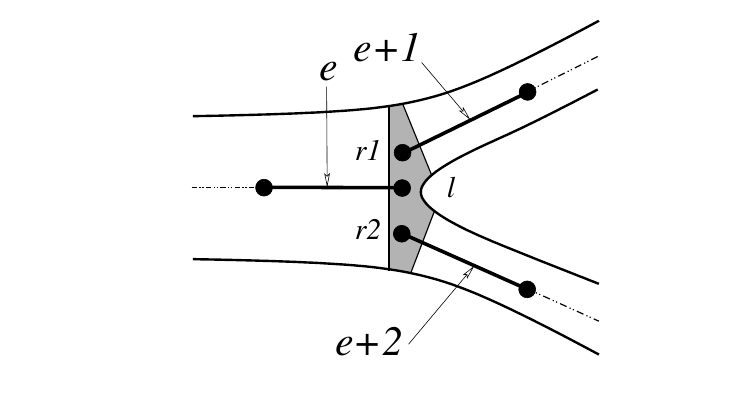
\includegraphics[width=0.5\linewidth]{arterial_tree_bifurcation.png}
    \caption{
Schematic representation of a Y-shaped arterial junction.
Element $e$ denotes the parent vessel, while elements $e+1$ and $e+2$ correspond
to the two daughter vessels.
The junction point is treated as a non-manifold interface in the DG
discretization, where mass conservation, pressure continuity, and
characteristic compatibility conditions are enforced.
}
\label{fig:arterial-tree}
\end{figure}
\paragraph{Junction conditions}
At each junction, six algebraic conditions are imposed to determine the unknown
junction states $(A_p,U_p,A_{d_1},U_{d_1},A_{d_2},U_{d_2})$.
These conditions consist of mass conservation, total pressure continuity, and
characteristic compatibility.
\begin{itemize}
    \item Mass conservation 
    \begin{equation}\label{eq:junction-mass}
A_p U_p = A_{d_1} U_{d_1} + A_{d_2} U_{d_2}. 
\end{equation}
\item Pressure continuity (bernoulli equation)
\begin{align}
\frac{U_p^2}{2} + P(A_p)
&=
\frac{U_{d_1}^2}{2} + P(A_{d_1}),
\label{eq:junction-pressure1}\\
\frac{U_p^2}{2} + P(A_p)
&=
\frac{U_{d_2}^2}{2} + P(A_{d_2}).
\label{eq:junction-pressure2}
\end{align}
\item Characteristic Compatibility: 
To close the system, characteristic compatibility conditions are imposed using
incoming Riemann invariants.
Let
\[
c(A) = \sqrt{\frac{A}{\rho}\frac{dP}{dA}(A)}
\]
denote the local wave speed.
The characteristic invariants are frozen from the previous time level and read
\begin{align}
U_p - 4 c(A_p) &= W_p^-,
\label{eq:junction-char-parent}\\
U_{d_1} + 4 c(A_{d_1}) &= W_{d_1}^+,
\label{eq:junction-char-d1}\\
U_{d_2} + 4 c(A_{d_2}) &= W_{d_2}^+,
\label{eq:junction-char-d2}
\end{align}
where $W_p^-$, $W_{d_1}^+$, and $W_{d_2}^+$ are computed from the solution at the
previous time step.
\end{itemize}
\subsection{Nonlinear Jacobian system for junction}

Equations \eqref{eq:junction-mass}--\eqref{eq:junction-char-d2} define a nonlinear
system of six equations for the six unknown junction states.
This system is solved locally at each junction using a Newton iteration,
initialized with the DG traces at the current time level.\\
The Jacobian matrix is assembled analytically by differentiating the junction
residuals with respect to the junction unknowns.
This local Jacobian is used both in the Newton solve of the junction system and
to consistently inject the junction contribution into the global DG Jacobian.

\subsection{Jacobian of the junction residual}

At a Y-shaped arterial junction, we collect the unknown junction states into the
vector
\[
\mathbf{X}
=
\begin{pmatrix}
A_p & U_p & A_{d_1} & U_{d_1} & A_{d_2} & U_{d_2}
\end{pmatrix}^{\!\top},
\]
where $(A_p,U_p)$ denote the area and velocity in the parent vessel, and
$(A_{d_1},U_{d_1})$, $(A_{d_2},U_{d_2})$ those in the two daughter vessels.

%------------------------------------------------------------
\paragraph{Junction residual.}

The nonlinear residual vector $\mathbf{R}(\mathbf{X}) \in \mathbb{R}^6$ is defined
componentwise as
\begin{align}
R_1 &= A_p U_p - A_{d_1} U_{d_1} - A_{d_2} U_{d_2},
\label{eq:junction-R1}\\
R_2 &= \tfrac12 U_p^2 + P(A_p)
      - \tfrac12 U_{d_1}^2 - P(A_{d_1}),
\label{eq:junction-R2}\\
R_3 &= \tfrac12 U_p^2 + P(A_p)
      - \tfrac12 U_{d_2}^2 - P(A_{d_2}),
\label{eq:junction-R3}\\
R_4 &= U_p - 4\,c(A_p) - W_p^{-},
\label{eq:junction-R4}\\
R_5 &= U_{d_1} + 4\,c(A_{d_1}) - W_{d_1}^{+},
\label{eq:junction-R5}\\
R_6 &= U_{d_2} + 4\,c(A_{d_2}) - W_{d_2}^{+},
\label{eq:junction-R6}
\end{align}
where
\[
c(A) = \sqrt{\frac{A}{\rho}\frac{dP}{dA}(A)}
\]
is the local wave speed, and $W_p^{-}$, $W_{d_1}^{+}$, $W_{d_2}^{+}$ denote the
incoming characteristic invariants frozen from the previous time level.

%------------------------------------------------------------
\paragraph{Jacobian matrix.}

The Jacobian matrix required for the Newton iteration is given by
\[
\mathbf{J}
=
\frac{\partial \mathbf{R}}{\partial \mathbf{X}}
=
\left[
\frac{\partial R_i}{\partial X_j}
\right]_{i,j=1}^{6}.
\]
Using
\[
\frac{dc}{dA}
=
\frac{1}{2c(A)}\,\frac{dP}{dA}(A),
\]
the Jacobian can be written explicitly as
\begin{equation}\label{eq:junction-jacobian}
\boxed{
\mathbf{J}
=
\begin{pmatrix}
U_p & A_p & -U_{d_1} & -A_{d_1} & -U_{d_2} & -A_{d_2} \\[2mm]

\dfrac{dP}{dA}(A_p) & U_p
& -\dfrac{dP}{dA}(A_{d_1}) & -U_{d_1}
& 0 & 0 \\[3mm]

\dfrac{dP}{dA}(A_p) & U_p
& 0 & 0
& -\dfrac{dP}{dA}(A_{d_2}) & -U_{d_2} \\[3mm]

-\dfrac{2}{c_p}\dfrac{dP}{dA}(A_p) & 1
& 0 & 0
& 0 & 0 \\[3mm]

0 & 0
& \dfrac{2}{c_{d_1}}\dfrac{dP}{dA}(A_{d_1}) & 1
& 0 & 0 \\[3mm]

0 & 0
& 0 & 0
& \dfrac{2}{c_{d_2}}\dfrac{dP}{dA}(A_{d_2}) & 1
\end{pmatrix}
}
\end{equation}
where
\[
c_p = c(A_p), \qquad
c_{d_1} = c(A_{d_1}), \qquad
c_{d_2} = c(A_{d_2}).
\]

%------------------------------------------------------------
\paragraph{Remark.}

The Jacobian \eqref{eq:junction-jacobian} is assembled analytically and used both
to solve the local $6\times6$ nonlinear junction system and to inject the
junction contribution consistently into the global DG--Newton Jacobian matrix.


\begin{remark}
\begin{itemize}
\item {Newton update.}
Once the corrections $(\delta A_h^{n+1,(k)},\,\delta U_h^{n+1,(k)})$ are computed,
the iterates are updated as
\[
  A_h^{n+1,(k+1)} = A_h^{n+1,(k)} + \delta A_h^{n+1,(k)}, 
  \qquad
  U_h^{n+1,(k+1)} = U_h^{n+1,(k)} + \delta U_h^{n+1,(k)}.
\]
The process is repeated until 
$\|\delta\mathbf{W}_h^{n+1,(k)}\|$ falls below a prescribed tolerance.
\item The increment $\delta\mathbf{W}_h^{n+1,(k)}$ represents the Newton correction at
time level $t_{n+1}$ and iteration $k$, while the Jacobian
$\mathcal{J}^{(k)}$ is obtained by differentiating the discrete residual
$\mathcal{R}^{n+1}(\mathbf{W})$ with respect to $\mathbf{W}$.
The term $\mathbf{H}^{(k)}\delta\mathbf{W}_h^{n+1,(k)}$ originates from the
first-order Taylor expansion of the nonlinear flux
$\mathbf{F}(\mathbf{W})$ about $\mathbf{W}_h^{n+1,(k)}$.
\end{itemize}
\end{remark}

\clearpage
\section*{Appendix}
\addcontentsline{toc}{section}{Appendix}
\appendix
\paragraph{From book: \textit{Nodal Discontinuous Galerkin Methods:
Algorithms, Analysis, and Applications}}
\begin{remark}
\begin{itemize}
   \item $\textbf{Page}~29$. An important lesson to learn from this is that a visually smoother solution
is not necessarily a more accurate solution, although in the case considered
here, the global errors are comparable.
\item $\textbf{Page}~169$.  The dissipative nature of this flux will smear shocks in strongly supersonic $|u| > c$
and transitional flows but will serve adequately for most subsonic $|u| < c$ and weakly
supersonic flows ach number (\(M\)) is slightly greater than 1. The Mach number is the ratio of the flow speed (\(|u|\)) to the speed of sound (\(c\)), or \(M=|u|/c\).
\item $\textbf{Page}~169$. We assume that the correct number
of boundary conditions are available at all inflow points of the boundary, $\partial \Omega$
(i.e., where the eigenvalues of the flux-Jacobian, $\hat{n} \cdot f u$, are negative along the
outward-pointing normal,$\hat{n}$).
\end{itemize}
\end{remark}

\section{Number of inlet and outlet boundary condtions}
 $\textbf{Page}~33$. If we consider systems of conservation laws
\begin{equation}
    \frac{\partial u}{\partial t} + \frac{\partial f(u)}{\partial x} = 0,
    \qquad x \in [L,R],
    \label{eq:system-cons}
\end{equation}
with initial conditions
\begin{equation}
    u(x,0) = u_0(x),
\end{equation}
no essentially new component is introduced in order to obtain the
semi-discrete schemes. In this case, the unknown is an $m$-vector
\[
    u = \bigl(U_1(x,t),\ldots,u_m(x,t)\bigr)^{T},
\]
and the flux is a vector-valued function $f:\mathbb{R}^m \to \mathbb{R}^m$.

The question of boundary conditions---and, ultimately, the choice of
the numerical flux---is more complicated for systems than for scalar
problems. In general terms, the boundary conditions are written as
\begin{align}
    B_L\,u(L,t) &= g_1(t), \qquad \text{at } x = L, \\
    B_R\,u(R,t) &= g_2(t), \qquad \text{at } x = R,
\end{align}
where the sum of the ranks of the boundary operators $B_L$ and $B_R$
equals the required number of inflow conditions.
\item For a one-dimensional hyperbolic system
\[
u_t + f(u)_x = 0,
\]
with Jacobian \(A(u) = f'(u)\) and eigenvalues
\(\lambda_1(u),\dots,\lambda_m(u)\),
the sign of the projected characteristic speeds
\[
\lambda_i\, n
\]
determines the admissible boundary conditions at a boundary with outward
normal \(n\).

A characteristic field is \emph{incoming} if
\[
\lambda_i \, n < 0,
\]
and \emph{outgoing} if
\[
\lambda_i \, n > 0.
\]

Only the incoming fields require the prescription of boundary data.
Therefore, the number of boundary conditions equals the number of incoming
characteristics.  Equivalently, if \(B_L\) and \(B_R\) denote the boundary
operators at the left and right boundaries, then
\[
\operatorname{rank}(B_L)+\operatorname{rank}(B_R)
 = \text{number of incoming characteristic fields}.
\]

\section{Boundary treatment in the Newton linearization for LF flux}
\label{bd:Lf_flux}
This algorithm based on the paper \textit{Boundary conditions for hyperbolic systems of partial differentials equations} by \textit{Amr G. Guaily , Marcelo Epstein}.

At a boundary face $e \subset \partial\Omega$, the Newton linearization of the
Lax–Friedrichs flux requires replacing the exterior trace
$\mathbf{W}^+$ by a boundary state $\mathbf{W}_b$.
Because the blood–flow equations are hyperbolic, the number of boundary
conditions that must be imposed depends on the signs of the characteristic
speeds
\[
  \lambda_{1,2} = U \mp c , \qquad
  c = \sqrt{\frac{A}{\rho}\frac{dP}{dA}(A)} .
\]
The linearized numerical flux is
\[
\delta\widehat{\mathbf{F}}^{(k)}
=
\tfrac12\!\left(
\mathbf{H}^-\,\delta\mathbf{W}^- (b \cdot n)^{-} +
\mathbf{H}^+\,\delta\mathbf{W}^+ (b \cdot n)^{+}
\right)
-\tfrac12\alpha^{(k)}\,
  (\delta\mathbf{W}^+ - \delta\mathbf{W}^-),
\]
where the key question is how the boundary variation $\delta\mathbf{W}^+$ is
assigned.  
This depends on the flow regime and on whether the boundary is an inlet or
outlet.  We distinguish the three physically relevant cases.

% ===============================================================
\subsubsection{Subcritical flow (one incoming characteristic)}

Subcritical flow is characterised by one incoming and one outgoing
characteristic:
\[
  \lambda_1 < 0 < \lambda_2 .
\]
Hence exactly one scalar boundary condition is required; the other component
must be taken from the interior.

\paragraph{(a) Subcritical inlet ($x=0$).}
At an inlet, the incoming characteristic is associated with the area variable.
Thus
\[
  A^+ = A_b, \qquad U^+ = U^-,
\]
and therefore
\[
  \delta A^+ = 0, \qquad
  \delta U^+ = \delta U^- .
\]
Numerical Flux in residual becomes 
\begin{align*}
 \widehat{F}_A &= \tfrac{1}{2} (A^{+} U^{+}  + A^{-}U^{-})(b \cdot n) - \tfrac{\alpha}{2}(A^{+} - A^{-})\\
 & = \frac{1}{2}(A_b U^{-} + A^{-}U^{-}) - \tfrac{\alpha}{2}(A_b -A^{-}).\\
\widehat{F}_U &= \tfrac{1}{2} \left(\frac{(U^-)^2}{2} + \frac{1}{\rho}P(A^-) + \frac{(U^+)^2}{2} + \frac{1}{\rho}P(A^+)\right)(b \cdot n) -\tfrac{\alpha}{2}(U^+ - U^-) \\
& = \frac{1}{2}\left( (U^{-})^2 +\frac{1}{\rho} P(A^-)  + \frac{1}{\rho} P(A_b)   \right).
\end{align*}

The linearized numerical flux components become:
\[
\delta\widehat{F}_A
=
\tfrac12\left(U^-\,\delta A^- +A_b\,\delta U^-\right)(b \cdot n)
+ \tfrac12\alpha\delta A^-,
\]
\begin{align*}
\delta\widehat{F}_U
& =
\tfrac12\left(\frac{(c^-)^2}{A^-}\delta A^- + U^-\,\delta U^-\right)(b \cdot n) + \tfrac12\left(\frac{(c^+)^2}{A^+}\delta A^+ + U^+\,\delta U^+\right)(b \cdot n) - \tfrac\alpha2(\delta U^{+} - \delta U^{-}), \\
& = \tfrac12\left(\frac{(c^-)^2}{A^-}\delta A^- + 2 U^-\,\delta U^-\right)(b \cdot n).
\end{align*}

\paragraph{(b) Subcritical outlet ($x=L$).}
Here the incoming characteristic is associated with the momentum.
Hence
\[
  A^+ = A^-, \qquad U^+ = U_b,
\]
and therefore
\[
  \delta A^+ = \delta A^-, \qquad
  \delta U^+ = 0.
\]
Numerical Flux in residual becomes 
\begin{align*}
 \widehat{F}_A &= \tfrac{1}{2} (A^{+} U^{+}  + A^{-}U^{-})(b \cdot n) - \tfrac{\alpha}{2}(A^{+} - A^{-})\\
 & = \frac{1}{2}(A^{-} U_b + A^{-}U^{-}) .\\
\widehat{F}_U &= \tfrac{1}{2} \left(\frac{(U^-)^2}{2} + \frac{1}{\rho}P(A^-) + \frac{(U^+)^2}{2} + \frac{1}{\rho}P(A^+)\right)(b \cdot n) -\tfrac{\alpha}{2}(U^+ - U^-) \\
& = \frac{1}{2}\left( \frac{(U^-)^2}{2} +2 \frac{1}{\rho} P(A^-) + \frac{(U_b)^2}{2}\right) (b\cdot n) - \tfrac{\alpha}{2}(U_b -U^{-})).
\end{align*}

The linearized flux becomes
\begin{align*}
\delta\widehat{F}_A
&=
\tfrac12\left(U^-\,\delta A^- + A^-\,\delta U^-\right)(b \cdot n) + \tfrac12\left(U^+\,\delta A^+ + A^+\,\delta U^+\right)(b \cdot n) - \tfrac\alpha2 ( \delta A^+ - \delta A^{-})\\
& = \tfrac{1}{2}\left( U^-\,\delta A^- + A^-\,\delta U^- + U_b \delta A^-\right)(b\cdot n)
\end{align*}
\begin{align*}
\delta\widehat{F}_U
&=
\tfrac12\left(\frac{(c^{-})^2}{A^-}\delta A^- + U^-\,\delta U^-\right)(b \cdot n)+\tfrac12\left(\frac{(c^{+})^2}{A^+}\delta A^+ + U^+\,\delta U^+\right)(b \cdot n)
- \tfrac12\alpha\,(\delta U^+ - \delta U^{-}) ,\\
& = \tfrac12\left( 2 \frac{(c^{-})^2}{A^-}\delta A^- +  U^-\,\delta U^-\right) + \tfrac{\alpha}{2}\delta U^{-}
\end{align*}

% ===============================================================
\subsubsection{Supercritical inflow (two incoming characteristics)}

In this regime
\[
  \lambda_1 < 0,\qquad \lambda_2 < 0,
\]
both characteristics enter the domain, so \emph{both} components of the
boundary state must be prescribed:
\[
  A^+ = A_b, \qquad U^+ = U_b.
\]
Thus the variations vanish:
\[
  \delta A^+ = 0, \qquad \delta U^+ = 0.
\]

Numerical Flux in residual becomes 
\begin{align*}
 \widehat{F}_A &= \tfrac{1}{2} (A^{+} U^{+}  + A^{-}U^{-})(b \cdot n) - \tfrac{\alpha}{2}(A^{+} - A^{-})\\
 & = \frac{1}{2}(A_b U_b + A^{-}U^{-}) - \tfrac{\alpha}{2}(A_b - A^{-}).\\
\widehat{F}_U &= \tfrac{1}{2} \left(\frac{(U^-)^2}{2} + \frac{1}{\rho}P(A^-) + \frac{(U^+)^2}{2} + \frac{1}{\rho}P(A^+)\right)(b \cdot n) -\tfrac{\alpha}{2}(U^+ - U^-) \\
& = \frac{1}{2}\left( \frac{(U^-)^2}{2} +\frac{1}{\rho} P(A^-) + \frac{(U_b)^2}{2} +\frac{1}{\rho} P(A_b)\right) (b\cdot n) - \tfrac{\alpha}{2}(U_b -U^{-})).
\end{align*}

Hence no boundary degrees of freedom contribute to the Jacobian at such a face,
and
\[
\delta\widehat{F}_A
=
\tfrac12\left(U^-\,\delta A^- + A^-\,\delta U^-\right)
+ \tfrac12\alpha (\delta A^-),
\qquad
\delta\widehat{F}_U
=
\tfrac12\left(\frac{c^2}{A^-}\delta A^- + U^-\,\delta U^-\right)
+ \tfrac12\alpha (\delta U^-).
\]

% ===============================================================
\subsubsection{Supercritical outflow (two outgoing characteristics)}

Finally, when
\[
  \lambda_1 > 0,\qquad \lambda_2 > 0 ,
\]
all characteristics leave the domain, so no physical boundary condition is
imposed.  Thus
\[
  A^+ = A^-,\qquad U^+ = U^-,
\qquad\Longrightarrow\qquad
  \delta A^+ = \delta A^-,\quad
  \delta U^+ = \delta U^- .
\]
Numerical Flux in residual becomes 
\begin{align*}
 \widehat{F}_A &= \tfrac{1}{2} (A^{+} U^{+}  + A^{-}U^{-})(b \cdot n) - \tfrac{\alpha}{2}(A^{+} - A^{-})\\
 & = \frac{1}{2}( 2 A^{-}U^{-}).\\
\widehat{F}_U &= \tfrac{1}{2} \left(\frac{(U^-)^2}{2} + \frac{1}{\rho}P(A^-) + \frac{(U^+)^2}{2} + \frac{1}{\rho}P(A^+)\right)(b \cdot n) -\tfrac{\alpha}{2}(U^+ - U^-) \\
& = \frac{1}{2}\left( 2 \frac{(U^-)^2}{2} + 2\frac{1}{\rho} P(A^-) \right) (b\cdot n).
\end{align*}

In this case, the Lax--Friedrichs dissipation vanishes because
$\delta\mathbf{W}^+=\delta\mathbf{W}^-$, and the linearized flux reduces to
\[
\delta\widehat{\mathbf{F}}
=
\begin{pmatrix}
U^-\,\delta A^- + A^-\,\delta U^- \\[1mm]
\dfrac{c^2}{A^-}\,\delta A^- + U^-\,\delta U^-
\end{pmatrix}.
\]


\paragraph{Summary.}
The mapping for the exterior state and its Newton variation is summarised in
Table~\ref{tab:bd-newton}.

\begin{table}[h!]
\centering
\begin{tabular}{c|c|c|c}
\hline
\textbf{Flow regime} & $A^+$ & $U^+$ & $(\delta A^+,\,\delta U^+)$ \\ \hline
Subcritical inlet   & $A_b$  & $U^-$ & $(0,\ \delta U^-)$ \\[2mm]
Subcritical outlet  & $A^-$  & $U_b$ & $(\delta A^-,\ 0)$ \\[2mm]
Supercritical inflow & $A_b$ & $U_b$ & $(0,\ 0)$ \\[2mm]
Supercritical outflow & $A^-$ & $U^-$ & $(\delta A^-,\ \delta U^-)$ \\
\hline
\end{tabular}
\caption{Exterior state and Newton variation at boundaries.}
\label{tab:bd-newton}
\end{table}

\end{document}
